\chapter{Introduction}

\section{Motivation}
Revealing the structure of hierarchical organized data is a complex task where many approaches already exists (TODO cite). It is still an active research area as data scientists are facing ever greater challenges when analyzing large hierarchical datasets. One example is the Human Disease Network \cite{zhou_human_2014} which is a hierarchical network of disorders and disease genes with approximately 3000 nodes on two different hierarchy layers. Figure \ref{fig:Human_Disease_Network} shows us the representation of the data in a common two-dimensional layout where the classes of disorders are color coded. 
Depiction of hierarchical network structure in 2d faces us with many challenges: limitation of visual features, only two available axes for encoding spatial data and therefore limiting the ability of the user to detect clusters and lastly visualizing more than two layers. However, in other application areas like software engineering or social science we often face more than two hierarchical layers, so we need to find a way to handle these datasets. 

\cite{brath_3d_2014}

%Data scientists are facing ever greater challenges when analyzing large datasets with a hierarchical structure. 

\begin{figure}[h]
    \centering
    \begin{subfigure}[b]{0.4\columnwidth}
        \centering
        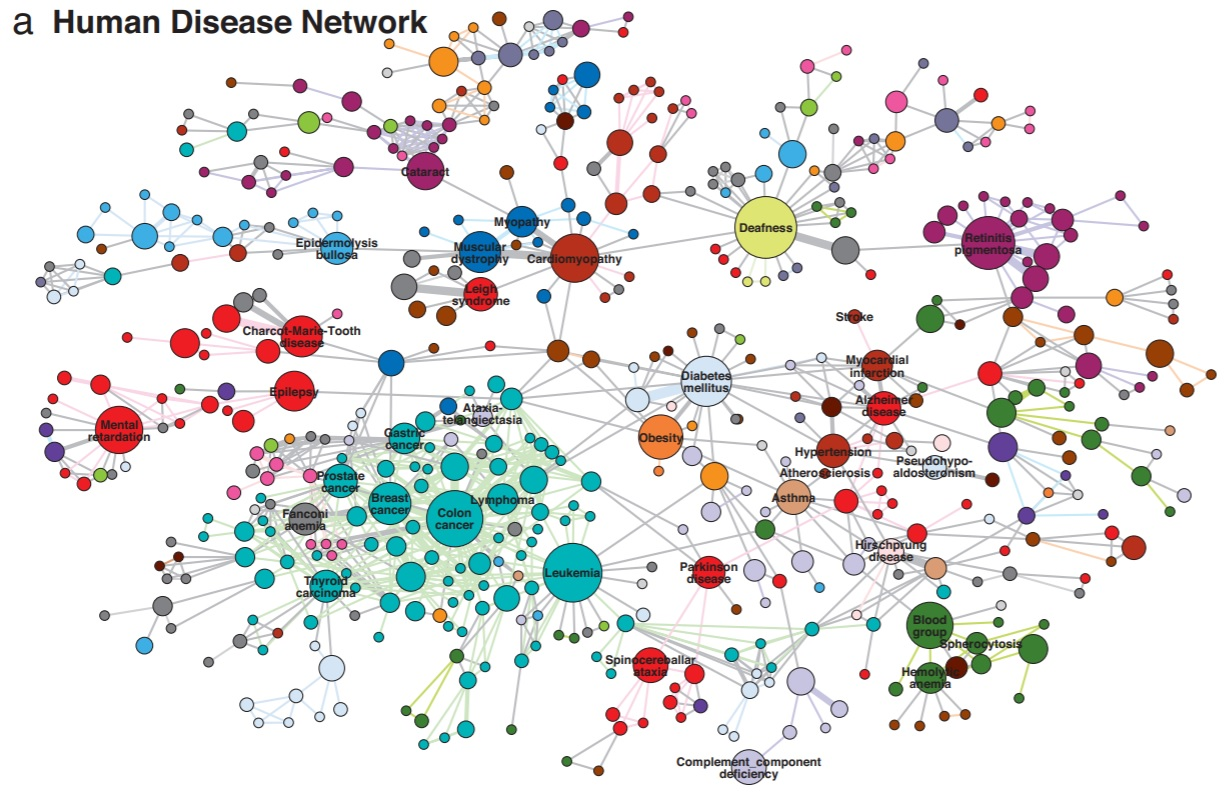
\includegraphics[width=\textwidth, trim={0 0 9cm 0},clip]{graphics/Human_Disease_Network.jpg}
        \subcaption{The Human Disease Network \cite{zhou_human_2014}}
        \label{fig:Human_Disease_Network}
    \end{subfigure}
    \begin{subfigure}[b]{0.5\columnwidth}
      \centering
      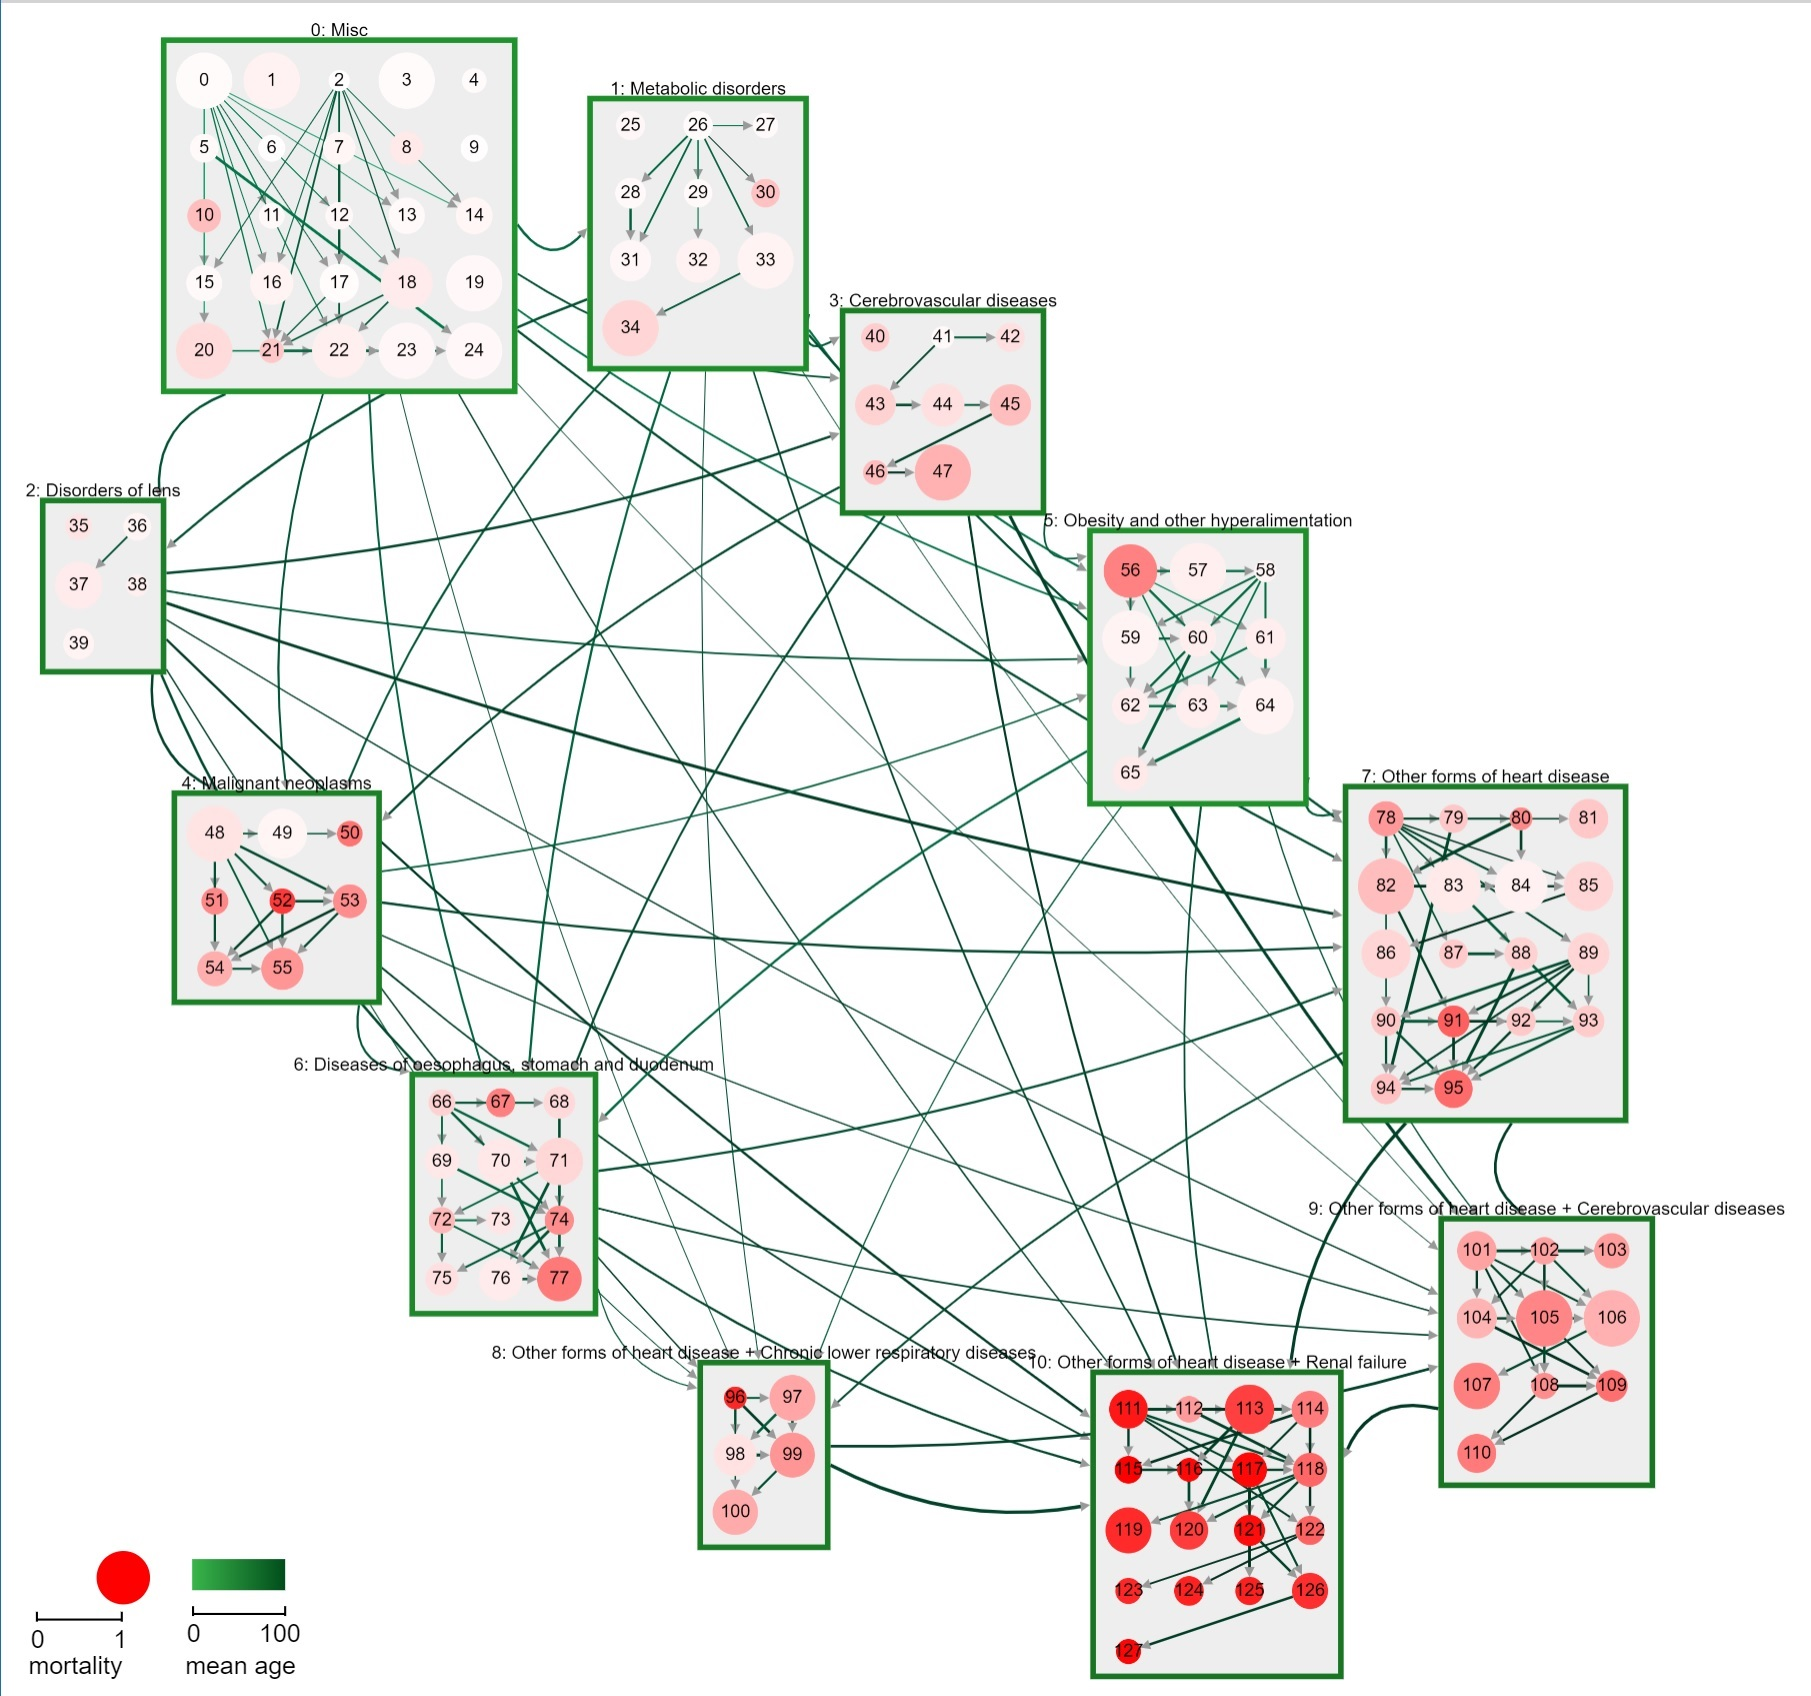
\includegraphics[width=\textwidth]{graphics/original2DdiseaseNet.jpg}
      \subcaption{Our own disease network dataset}
      \label{fig:original2DdiseaseNet}
    \end{subfigure}
    \caption[Optional caption for the figure list (often used to abbreviate long captions)]{Example visualizations of hierarchical network datasets in two dimensions. Both consists of two hierarchical layers.} % Remove the [...] argument if the original caption should be used in the figure list.
    \label{fig:intro} 
  \end{figure}




From proposal: \\
The	 goal	 is	 to	 visualize	 a	 hierarchical	 network	 with	 n	 Layers.	 Each	 Node	 in	 a	 graph	 can	
represent	a	graph	itself.	There	are	multiple	examples	where	this	has	been	visualised	in	2D,	
however	we	believe	that	with	an	additional	dimension	and	when	3D	graphs	are	analysed	in	
VR	we	can	get	even	more	insight	and	a	better	overview	of	the	data.	

\textbf{Starting idea: 2D Multilayer see figure, why not make use of all 3 axes in VR, instead of flat layers use 3D objects like cubes/spheres to bundle one layer} (Email 14.08.2020 https://arxiv.org/pdf/1902.06815.pdf)
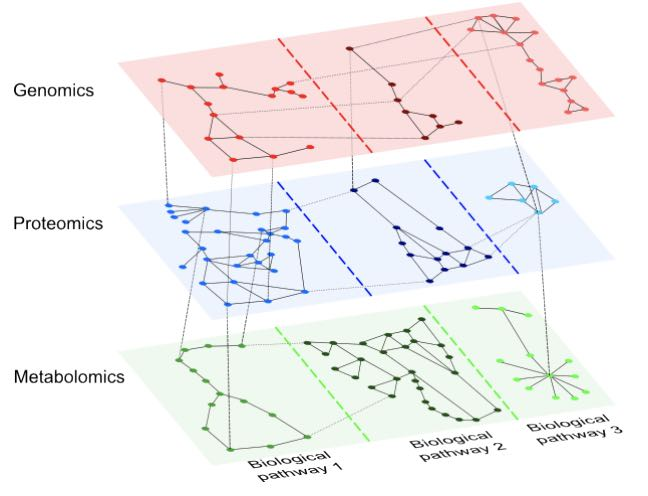
\includegraphics[width=0.5\textwidth]{chapters/graphics/2dmultilayerVis.jpg}

Ideas:
\begin{itemize}
    \item Example applications with hierarchical network data
    \item current 2D visualizations of hierarchical networks
    \item power of VR visualizations and board availability
\end{itemize}

\section{Aim of the Work}

Ideas:
\begin{itemize}
    \item provide a prototype application
    \item benefits of webbased implementation 
    \item experiment with different concepts/approaches
    \item experiment with different interactions
    \item ...
\end{itemize}

\begin{quotation}
    However, there is considerable value in research that
    solves a well-motivated problem using a combination
    of preexisting solutions 
\end{quotation}
Sadana\\
Redefining a Contribution for Immersive Visualization Research\\

\section{Approach}

I want to give a short summary of chapter 4 proposed solution here. 

Ideas:
\begin{itemize}
    \item short description of planned final solution (web based, htc vive compatible, rendering multi hierarchical dataset, screenshot of solution)  
    \item short overview of used technologies and frameworks why? what it simplifies, ... 
    \item Customized Forces
    \item rendering, nodes inside parent, comparison to a default 2D Circle Packing plot https://observablehq.com/@d3/zoomable-circle-packing 
    \item available interactions
\end{itemize}